% !TEX encoding = UTF-8
% !TEX program = pdflatex
% !TEX root = relazione-MEMOC.tex
% !TeX spellcheck = it_IT
\documentclass[a4paper, 11pt]{article} % Font size (can be 10pt, 11pt or 12pt) and paper size (remove a4paper for US letter paper)
\usepackage[italian]{babel}    							% Lingua italiana
\usepackage[margin=.9in]{geometry}             % Imposta i margini del documento

\usepackage[T1]{fontenc} % Required for accented characters
\usepackage[mathletters]{ucs}    % Caratteri matematici come UTF8
\usepackage[utf8,utf8x]{inputenc}      % Ancora utf8

\usepackage{eurosym}                %simbolo dell'euro
\usepackage[usenames,dvipsnames,svgnames,table]{xcolor}
\usepackage{listings}
% Imposta lo spazio nella list of listing in modo simile alla list of figures/tables
%\makeatletter
%\let\my@chapter\@chapter
%\renewcommand*{\@chapter}{%
%  \addtocontents{lol}{\protect\addvspace{10pt}}%
%  \my@chapter}
%\makeatother


\definecolor{codegreen}{rgb}{0,0.6,0}
\definecolor{codegray}{rgb}{0.5,0.5,0.5}
\definecolor{backcolor}{rgb}{0.98,0.98,0.98}

\renewcommand{\lstlistingname}{Codice}% Listing -> codice
\renewcommand{\lstlistlistingname}{Frammenti di codice}% List of Listings -> Frammenti di codice

\lstdefinestyle{mystyle}{
    backgroundcolor=\color{backcolor},   
    commentstyle=\color{Peach}\ttfamily,
    keywordstyle=\color{RoyalBlue},
    numberstyle=\tiny\color{codegray},
    stringstyle=\color{SeaGreen}\ttfamily,
    basicstyle=\footnotesize\ttfamily,
    breakatwhitespace=false,         
    breaklines=true,                 
    captionpos=b,                    
    keepspaces=true,                 
    numbers=left,                    
    numbersep=5pt,                  
    showspaces=false,                
    showstringspaces=false,
    showtabs=false,                  
    tabsize=2,
    frame=trbl, % draw a frame at the top, right, left and bottom of the listing
	frameround=ftff, % angolo in basso a destro curvo
	framesep=4pt, % quarter circle size of the round corners,
	inputencoding=utf8,
    extendedchars=true,
    literate={á}{{\'a}}1 {à}{{\`a}}1 {é}{{\'e}}1 {è}{{\`e}}1 {ù}{{\`u}}1 {ò}{{\`o}}1 {ì}{{\`i}}1,
    belowskip=1em,
    aboveskip=1em,
}

 
\lstset{style=mystyle}

\lstdefinelanguage{JavaScript}
{
  % list of keywords
  morekeywords={ true, false, catch, function, break,	new, class, extends, var, require, switch, return, import, if, while, for, this, View, Text, StyleSheet},
  sensitive=false, % keywords are not case-sensitive
  morecomment=[l]{//}, % l is for line comment
  morecomment=[s]{/*}{*/}, % s is for start and end delimiter
  morestring=[b]' % defines that strings are enclosed in double quotes
}

\lstdefinelanguage{Properties}
{
	% list of keywords
	morekeywords={ true, false, catch, function, break,	new, class, extends, var, require, switch, return, import, if, while, for, this, View, Text, StyleSheet},
	sensitive=false, % keywords are not case-sensitive
	morecomment=[l]{\#}, % l is for line comment
	morecomment=[s]{/*}{*/}, % s is for start and end delimiter
	morestring=[b]' % defines that strings are enclosed in double quotes
}

\lstdefinelanguage{JSON}
{
  % list of keywords
  morekeywords={string, boolean, int, Array, Node, Asset, AssetDetail, Filter, FilterItem},
  sensitive=false, % keywords are not case-sensitive
  morecomment=[l]{//}, % l is for line comment
  morecomment=[s]{/*}{*/}, % s is for start and end delimiter
  morestring=[b]" % defines that strings are enclosed in double quotes
}

\lstdefinelanguage{URM}
{
	% list of keywords
	morekeywords={ S, J, T, Z, I},
	sensitive=false, % keywords are not case-sensitive
	morecomment=[l]{//}, % l is for line comment
	morecomment=[s]{/*}{*/}, % s is for start and end delimiter
	morestring=[b]' % defines that strings are enclosed in double quotes
}

\lstdefinelanguage{RDFA}{
	language=html,
	sensitive=true, 
	alsoletter={<>=-},
	ndkeywords={
		% General
		=,
		% HTML attributes
		charset=, id=, width=, height=, property=, about=, rel=, rev=, prefix=, vocab=, content=, datatype=
	},  
	morecomment=[s]{<!--}{-->},
	tag=[s]
}

% Inserisco questi 2 package altrimenti su windows non compila! 
\usepackage[T1]{fontenc}
\usepackage{lmodern}

%\tightlist per compatibilità con pandoc
\providecommand{\tightlist}{%
	\setlength{\itemsep}{0pt}\setlength{\parskip}{0pt}}


\usepackage[labelfont=bf]{caption}

\usepackage[protrusion=true,expansion=true]{microtype} % Better typography
\usepackage{graphicx} % Required for including pictures
\usepackage{wrapfig} % Allows in-line images

\usepackage{multirow} 
\usepackage{subfig}
\usepackage{hyperref}
\usepackage{placeins}
\usepackage[scaled=0.8]{sourcecodepro}
\usepackage{hyperref}                   % collegamenti ipertestuali
\hypersetup{
	%hyperfootnotes=false,
	%pdfpagelabels,
	%draft,	% = elimina tutti i link (utile per stampe in bianco e nero)
	colorlinks=true,
	linktocpage=true,
	pdfstartpage=1,
	pdfstartview=FitV,
	% decommenta la riga seguente per avere link in nero (per esempio per la stampa in bianco e nero)
	%colorlinks=false, linktocpage=false, pdfborder={0 0 0}, pdfstartpage=1, pdfstartview=FitV,
	breaklinks=true,
	pdfpagemode=UseNone,
	pageanchor=true,
	pdfpagemode=UseOutlines,
	plainpages=false,
	bookmarksnumbered,
	bookmarksopen=true,
	bookmarksopenlevel=1,
	hypertexnames=true,
	pdfhighlight=/O,
	%nesting=true,
	%frenchlinks,
	urlcolor=Cerulean,
	linkcolor=RoyalBlue,
	citecolor=Cerulean,
	%pagecolor=RoyalBlue,
	%urlcolor=Black, linkcolor=Black, citecolor=Black, %pagecolor=Black,
	pdfsubject={},
	pdfkeywords={},
	pdfcreator={pdfLaTeX},
	pdfproducer={LaTeX}
}

\usepackage[colorinlistoftodos,prependcaption]{todonotes} %todo

\usepackage{amsmath}
\usepackage{mathtools}

\usepackage{float}
\usepackage{algorithm}
\usepackage{algpseudocode} % https://en.wikibooks.org/wiki/LaTeX/Algorithms#Typesetting_using_the_algorithmicx_package
\usepackage{amssymb}  %$\mathbb{N}$ per il simbolo dei numeri naturali 

\usepackage{enumerate} % permette di personalizzare enumerate

\usepackage{xmpincl}	%Aggiunge metadati sulla licenza CC
\usepackage{xspace}

\usepackage{bussproofs}

\makeatletter
\renewcommand\@biblabel[1]{\textbf{#1.}} % Change the square brackets for each bibliography item from '[1]' to '1.'
\renewcommand{\@listI}{\itemsep=0pt} % Reduce the space between items in the itemize and enumerate environments and the bibliography

\renewcommand{\maketitle}{ % Customize the title - do not edit title and author name here, see the TITLE block below
	\begin{flushright} % Right align
		{\LARGE\@title} % Increase the font size of the title
		
		\vspace{50pt} % Some vertical space between the title and author name
		
		{\large\@author} % Author name
		\\\@date % Date
		
		\vspace{100pt} % Some vertical space between the author block and abstract
	\end{flushright}
}

%% breakablealgorithm http://tex.stackexchange.com/questions/33866/algorithm-tag-and-page-break
\makeatletter
\newenvironment{breakablealgorithm}
{% \begin{breakablealgorithm}
	\begin{center}
		\refstepcounter{algorithm}% New algorithm
		\hrule height.8pt depth0pt \kern2pt% \@fs@pre for \@fs@ruled
		\renewcommand{\caption}[2][\relax]{% Make a new \caption
			{\raggedright\textbf{\ALG@name~\thealgorithm} ##2\par}%
			\ifx\relax##1\relax % #1 is \relax
			\addcontentsline{loa}{algorithm}{\protect\numberline{\thealgorithm}##2}%
			\else % #1 is not \relax
			\addcontentsline{loa}{algorithm}{\protect\numberline{\thealgorithm}##1}%
			\fi
			\kern2pt\hrule\kern2pt
		}
	}{% \end{breakablealgorithm}
	\kern2pt\hrule\relax% \@fs@post for \@fs@ruled
\end{center}
}
\makeatother

\makeatletter % trattino con punto sopra
\newcommand{\dotminus}{\mathbin{\text{\@dotminus}}}

\newcommand{\@dotminus}{%
	\ooalign{\hidewidth\raise1ex\hbox{.}\hidewidth\cr$\m@th-$\cr}%
}
\makeatother

\DeclarePairedDelimiter{\ceil}{\lceil}{\rceil}
\DeclarePairedDelimiter{\floor}{\lfloor}{\rfloor}


\let\oldtext\text



%----------------------------------------------------------------------------------------
% TITLE
%----------------------------------------------------------------------------------------
\begin{document}
%**************************************************************
% Frontespizio 
%**************************************************************
\begin{titlepage}
	
	\begin{center}
		
		\begin{LARGE}
			\textbf{Università degli Studi di Padova}\\
		\end{LARGE}
		
		\vspace{10pt}
		
		\begin{Large}
			\textsc{Dipartimento di Matematica}\\
		\end{Large}
		
		\vspace{10pt}
		
		\begin{large}
			\textsc{Corso di Laurea Magistrale in Informatica}\\
		\end{large}
		
		\vspace{30pt}
		\begin{figure}[htbp]
			\begin{center}
				
\includegraphics[height=6cm]{immagini/logo-unipd}
			\end{center}
		\end{figure}
		\vspace{10pt} 
		
		\begin{LARGE}
			\begin{center}
				\textbf{Relazione esercitazioni laboratorio}\\
			\end{center}
		\end{LARGE}
		
		\vspace{10pt} 
		
		\vspace{60pt} 
		
		\begin{large}
			%\begin{flushleft}
			%	\textit{Relatore}\\ 
			%	\vspace{5pt} 
		 	%	Prof. CEP
			%\end{flushleft}
			
			\begin{flushright}
				\textit{Autore}\\ 
				\vspace{5pt} 
				Giacomo Manzoli 1130822
			\end{flushright}
		\end{large}
		
		\vspace{160pt}
		
		\line(1, 0){338} \\
		\begin{normalsize}
			\textsc{Anno Accademico 2016-2017}
		\end{normalsize}
		
	\end{center}
\end{titlepage} 

%----------------------------------------------------------------------------------------


%----------------------------------------------------------------------------------------
%	DOCUMENT HEADER
%----------------------------------------------------------------------------------------


	%----------------------------------------------------------------------------------------
	% ABSTRACT AND KEYWORDS
	%----------------------------------------------------------------------------------------
	
	%\renewcommand{\abstractname}{Summary} % Uncomment to change the name of the abstract to something else
	
	\clearpage
	\tableofcontents
	
	%\hspace*{3,6mm}\textit{Keywords:} lorem , ipsum , dolor , sit amet , lectus % Keywords
	
	%\vspace{30pt} % Some vertical space between the abstract and first section
	
	%----------------------------------------------------------------------------------------
	% ESSAY BODY
	%----------------------------------------------------------------------------------------
	\clearpage
	% !TEX encoding = UTF-8
% !TEX program = pdflatex
% !TEX root = relazione-MEMOC.tex
% !TeX spellcheck = it_IT

\section{Introduzione}

L'obiettivo della prima parte del progetto è quello di implementare un modello in CPLEX e di provarlo in modo da trovare la dimensione massima del problema che permette una risoluzione esatta entro un certo limite di tempo, mentre la seconda parte prevede l'implementazione di un algoritmo meta-euristico ad-hoc per il problema e per poi confrontarlo con il modello CPLEX.

La sezione §\ref{sec:cplex} contiene la descrizione dell'implementazione del modello CPLEX con i relativi test, mentre la sezione §\ref{sec:genetico} contiene la descrizione dell'algoritmo genetico implementato e un confronto delle prestazioni rispetto a quelle ottenute da CPLEX.

\subsection{Generazione delle istanze}

Prima di implementare i vari algoritmi è stato necessario creare delle istanze per il problema.
\`E stato quindi creato uno script in Python in grado di generare delle istanze casuali a partire da un numero di nodi o fori.

Dato che il problema ha delle caratteristiche specifiche, ovvero visto che si tratta di schede perforate, è ragionevole assumere che i fori seguano un certo pattern.
Pertanto lo script è stato sviluppato in modo che possa generare anche delle istanze pseudo-casuali, ovvero delle istanze in cui ci sono blocchi di punti che compaiono vicini tra loro, raggruppati in rettangoli e a coppie.

In entrambi i casi, una volta generati i punti, le distanze sono state calcolate utilizzando la distanza euclidea.

\begin{figure}[htbp]
	\centering
	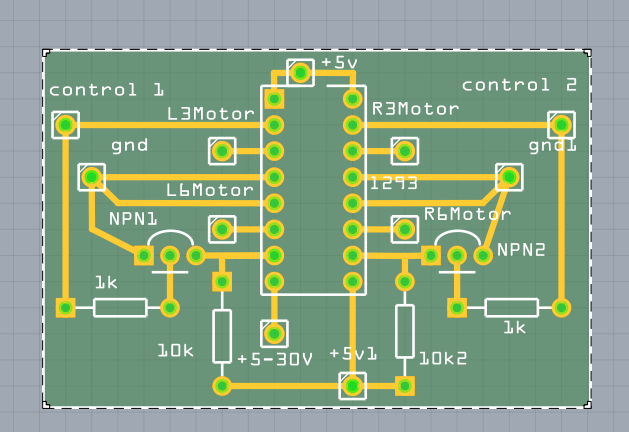
\includegraphics[width=.5\textwidth]{immagini/scheda.png}
	\caption{Esempio di scheda perforata presa come riferimento per la generazione delle istanze pseudo-casuali.}
\end{figure}	% Introduzione
	% !TEX encoding = UTF-8
% !TEX program = pdflatex
% !TEX root = relazione-MEMOC.tex
% !TeX spellcheck = it_IT

\section{CPLEX} \label{sec:cplex}

Il modello CPLEX è stato implementato come specificato nella consegna della prima esercitazione con dei particolari accorgimenti per rendere il codice più comprensibile e mantenibile:

\begin{itemize}
	\item Le informazioni relative al problema e ad una sua possibile soluzione sono state modellate con due classi \texttt{Problem} e \texttt{Solution}. Inoltre, tutta la logica di risoluzione è stata incapsulata nella classe \texttt{CPLEXSolver}.
	\item Durante la dichiarazione delle variabili viene costruita una mappa di supporto per rendere più agevole l'utilizzo delle variabili all'interno dei vincoli. Viene inoltre limitato il numero di variabili, evitando di definire le variabili $x_{ii}$ e $y_{ii}$.
	\item I vincoli vengono definiti uno alla volta, in modo da semplificare la sintassi di definizione.
\end{itemize}

\subsection{Definizione delle variabili}

Le variabili in CPLEX, una volta create, vengono memorizzate in sequenza all'interno di un array interno del risolutore e l'unico modo per riferirsi ad una variabile è mediante la sua posizione nell'array interno.

Per riferirsi più facilmente alle variabili, viene quindi creata una matrice di dimensione $N\times N$ che associa il ``\textit{nome della variabile}'' alla sua posizione interna nel risolutore.

\begin{lstlisting}[language=C++, caption=Creazione delle variabili $x_{ij}$]
// xMap[i][j] è una matrice N x N
for (int i = 0; i < N; ++i) {
	for (int j = 0; j < N; ++j) {
		if (i == j) continue;
		char htype = 'I';
		double obj = 0.0;
		double lb = 0.0;
		double ub = CPX_INFBOUND;
		snprintf(name, NAME_SIZE, "x_%d,%d", nodes[i], nodes[j]);
		char* xname = &name[0];
		CHECKED_CPX_CALL( CPXnewcols, env, lp, 1, &obj, &lb, &ub, &htype, &xname );
		xMap[i][j] = createdVars;
		createdVars++;
	}
}
\end{lstlisting}

\noindent La mappatura del nome viene fatta nella riga 12 del frammento: \texttt{createdVars} è una variabile che tiene traccia del numero di variabili che sono state create nel risolutore e quindi la prossima variabile aggiunta avrà come indice interno il valore di \texttt{createdVars}. Il valore dell'indice viene quindi memorizzato nella mappa e poi incrementato, in modo che alla successiva iterazione dei ciclo, questo sia ancora corretto.

Nello stesso frammento di codice è possibile osservare come \textbf{non} vengano create le variabili $x_{ii}$, questo perché quando i due indici sono uguali, l'\texttt{if} in riga 4 blocca l'esecuzione del corpo. 
Questa scelta è stata fatta perché tale variabile non è significativa per il problema, in quanto scegliere di spostare la trivella lungo l'arco $(i,i)$ equivale al lasciare ferma la trivella.

Quanto riportato è stato effettuato anche per le variabili $y_{ij}$.

\subsection{Definizione dei vincoli}

CPLEX permette di definire più vincoli con una sola istruzione, tuttavia la notazione per sfruttare questa possibilità è poco pratica da usare, in quanto richiede che gli indici delle variabili e i corrispettivi coefficienti vengano passati come una matrice sparsa, linearizzata in un vettore.
Se invece viene creato un vincolo alla volta, non c'è la necessità di gestire la matrice sparsa, in quanto questa è composta da una sola riga e quindi può essere considerata come vettore. 
Detto in altre parole, non è necessario utilizzare il vettore \texttt{rmatbeg} per tenere traccia dell'inizio delle varie righe, dato che essendoci un'unica riga, questa inizierà alla posizione 0 degli array utilizzati per definire il vincolo.

\begin{lstlisting}[language=C++, caption=Esempio di creazione di una serie di vincoli]
// Vincoli sul flusso in ingresso
for (int j = 0; j < N; ++j){
	std::vector<int> varIndex(N-1);
	std::vector<double> coef(N-1);
	int idx = 0;
	// Recupero gli indici dalla mappa delle varibaili
	for (int i = 0; i < N; ++i) {
		if (i==j) continue;
		varIndex[idx] = yMap[i][j];
		coef[idx] = 1;
		idx++;
	}
	char sense = 'E';
	double rhs = 1;
	snprintf(name, NAME_SIZE, "in_%d",j+1);
	char* cname = (char*)(&name[0]);

	int matbeg = 0;
	CHECKED_CPX_CALL( CPXaddrows, env, lp, 
						0, // Numero di variabili da creare
						1, // Numero di vincoli da creare
						varIndex.size(), // Numero di variabili nel vincolo con coeff != 0
						&rhs, // Parte destra del vincolo
						&sense, // Senso
						&matbeg, // 0 perché creo un solo vincolo
						&varIndex[0], // Inizio dell'array con gli indici delle variabili
						&coef[0], // Inizio dell'array con i coefficienti delle variabili
						NULL,  // Nomi per le nuove variabili
						&cname // Nome del vincolo
					);
}
\end{lstlisting}

\noindent Dal codice sopra riportato si può osservare come la chiamata della riga 19 definisce solamente un vincolo, pertanto per generare tutti vincoli del tipo

$$
\sum\limits_{j : (i,j) \in A} y_{ij} = 1 \quad \forall j \in N
$$

\noindent è necessario effettuare un iterazione esterna con il ciclo \texttt{for} di riga 2.

Questo modo di definire i vincoli potrebbe essere leggermente meno efficiente, dato che effettua più chiamate ai metodi del risolutore, ma l'impatto sulle prestazioni rimane comunque basso, dato che i vincoli vengono creati solamente all'inizializzazione del modello e il tempo necessario è molto inferiore rispetto a quello necessario per l'ottimizzazione.

\subsection{Test del modello}

\`E stato richiesto di osservare qual'è la dimensione massima di un problema che il modello CPLEX riesce a risolvere entro un certo periodo di tempo.

Per fare ciò sono state prima generate 5 istanze casuali e 5 pseudo casuali per ogni dimensione $5$, $10$, $\ldots$, $100$ ed è stato eseguito CPLEX con un time limit di 10 minuti. Sono stati poi presi in considerazione 4 livelli di time limit: un secondo, dieci secondi, un minuto e dieci minuti ed è stato osservato qual'è la massima dimensione che può essere risolta entro tali intervalli.
I risultati medi delle esecuzioni sulle istanze di varie dimensioni sono riportati nella tabella \ref{tab:cplex-avg} e riassunti nel grafico \ref{fig:cplex-time}, mentre la corrispondenza time limit/difficoltà massima è riassunta nella tabella \ref{tab:cplex-recap}.

\begin{table}[htbp]
	\centering
	\resizebox{\textwidth}{!}{%
		\begin{tabular}{c|c|c|c|c|c|c|c|c|}
			\cline{2-9}
			\multicolumn{1}{l|}{} & \multicolumn{4}{c|}{\textbf{Pseudo}} & \multicolumn{4}{c|}{\textbf{Random}} \\ \hline
			\multicolumn{1}{|l|}{\textbf{Dimensione}} & \multicolumn{1}{l|}{\textbf{\begin{tabular}[c]{@{}l@{}}Tempo \\ medio\end{tabular}}} & \multicolumn{1}{l|}{\textbf{\begin{tabular}[c]{@{}l@{}}Tempo\\ minimo\end{tabular}}} & \multicolumn{1}{l|}{\textbf{\begin{tabular}[c]{@{}l@{}}Tempo\\ massimo\end{tabular}}} & \multicolumn{1}{l|}{\textbf{Fallimenti}} & \multicolumn{1}{l|}{\textbf{\begin{tabular}[c]{@{}l@{}}Tempo\\ medio\end{tabular}}} & \multicolumn{1}{l|}{\textbf{\begin{tabular}[c]{@{}l@{}}Tempo\\ minimo\end{tabular}}} & \multicolumn{1}{l|}{\textbf{\begin{tabular}[c]{@{}l@{}}Tempo\\ massimo\end{tabular}}} & \multicolumn{1}{l|}{\textbf{Fallimenti}} \\ \hline
			\multicolumn{1}{|c|}{5} & 0,02 & 0,01 & 0,04 & 0 & 0,02 & 0,01 & 0,04 & 0 \\ \hline
			\multicolumn{1}{|c|}{10} & 0,08 & 0,04 & 0,14 & 0 & 0,06 & 0,03 & 0,08 & 0 \\ \hline
			\multicolumn{1}{|c|}{15} & 0,14 & 0,06 & 0,23 & 0 & 0,20 & 0,09 & 0,31 & 0 \\ \hline
			\multicolumn{1}{|c|}{20} & 0,82 & 0,10 & 1,88 & 0 & 0,46 & 0,28 & 0,65 & 0 \\ \hline
			\multicolumn{1}{|c|}{25} & 1,38 & 0,17 & 3,88 & 0 & 0,92 & 0,43 & 1,57 & 0 \\ \hline
			\multicolumn{1}{|c|}{30} & 3,51 & 0,16 & 6,80 & 0 & 2,03 & 0,88 & 4,27 & 0 \\ \hline
			\multicolumn{1}{|c|}{35} & 4,75 & 0,52 & 11,94 & 0 & 3,87 & 1,47 & 6,87 & 0 \\ \hline
			\multicolumn{1}{|c|}{40} & 129,16 & 0,03 & 600,04 & 1 & 6,53 & 2,32 & 9,03 & 0 \\ \hline
			\multicolumn{1}{|c|}{45} & 31,50 & 5,01 & 94,31 & 0 & 10,22 & 9,11 & 12,89 & 0 \\ \hline
			\multicolumn{1}{|c|}{50} & 114,99 & 18,88 & 350,22 & 0 & 18,16 & 13,72 & 24,37 & 0 \\ \hline
			\multicolumn{1}{|c|}{55} & 36,53 & 26,39 & 47,00 & 0 & 24,98 & 15,83 & 53,49 & 0 \\ \hline
			\multicolumn{1}{|c|}{60} & 52,91 & 28,03 & 77,75 & 0 & 42,82 & 23,03 & 73,45 & 0 \\ \hline
			\multicolumn{1}{|c|}{65} & 215,51 & 55,89 & 600,08 & 1 & 81,70 & 62,26 & 119,60 & 0 \\ \hline
			\multicolumn{1}{|c|}{70} & 196,50 & 60,60 & 600,08 & 1 & 62,39 & 35,62 & 91,72 & 0 \\ \hline
			\multicolumn{1}{|c|}{75} & 239,86 & 6,97 & 411,80 & 0 & 90,25 & 48,40 & 114,86 & 0 \\ \hline
			\multicolumn{1}{|c|}{80} & 318,38 & 57,05 & 600,10 & 2 & 203,84 & 89,87 & 399,65 & 0 \\ \hline
			\multicolumn{1}{|c|}{85} & 245,64 & 93,26 & 600,14 & 1 & 268,20 & 69,19 & 550,24 & 0 \\ \hline
			\multicolumn{1}{|c|}{90} & 474,56 & 207,08 & 600,17 & 3 & 311,61 & 155,87 & 600,13 & 1 \\ \hline
			\multicolumn{1}{|c|}{95} & 517,15 & 185,08 & 600,20 & 4 & 445,41 & 238,19 & 600,20 & 1 \\ \hline
		\end{tabular}%
	}
	\caption{Risultatati medi dell'esecuzione del risolutore CPLEX su 5 istanze diverse per ogni dimensione. Tutti i tempi riportati nella tabella sono espressi in secondi.}
	\label{tab:cplex-avg}
\end{table}

\begin{figure}[htbp]
	\centering
	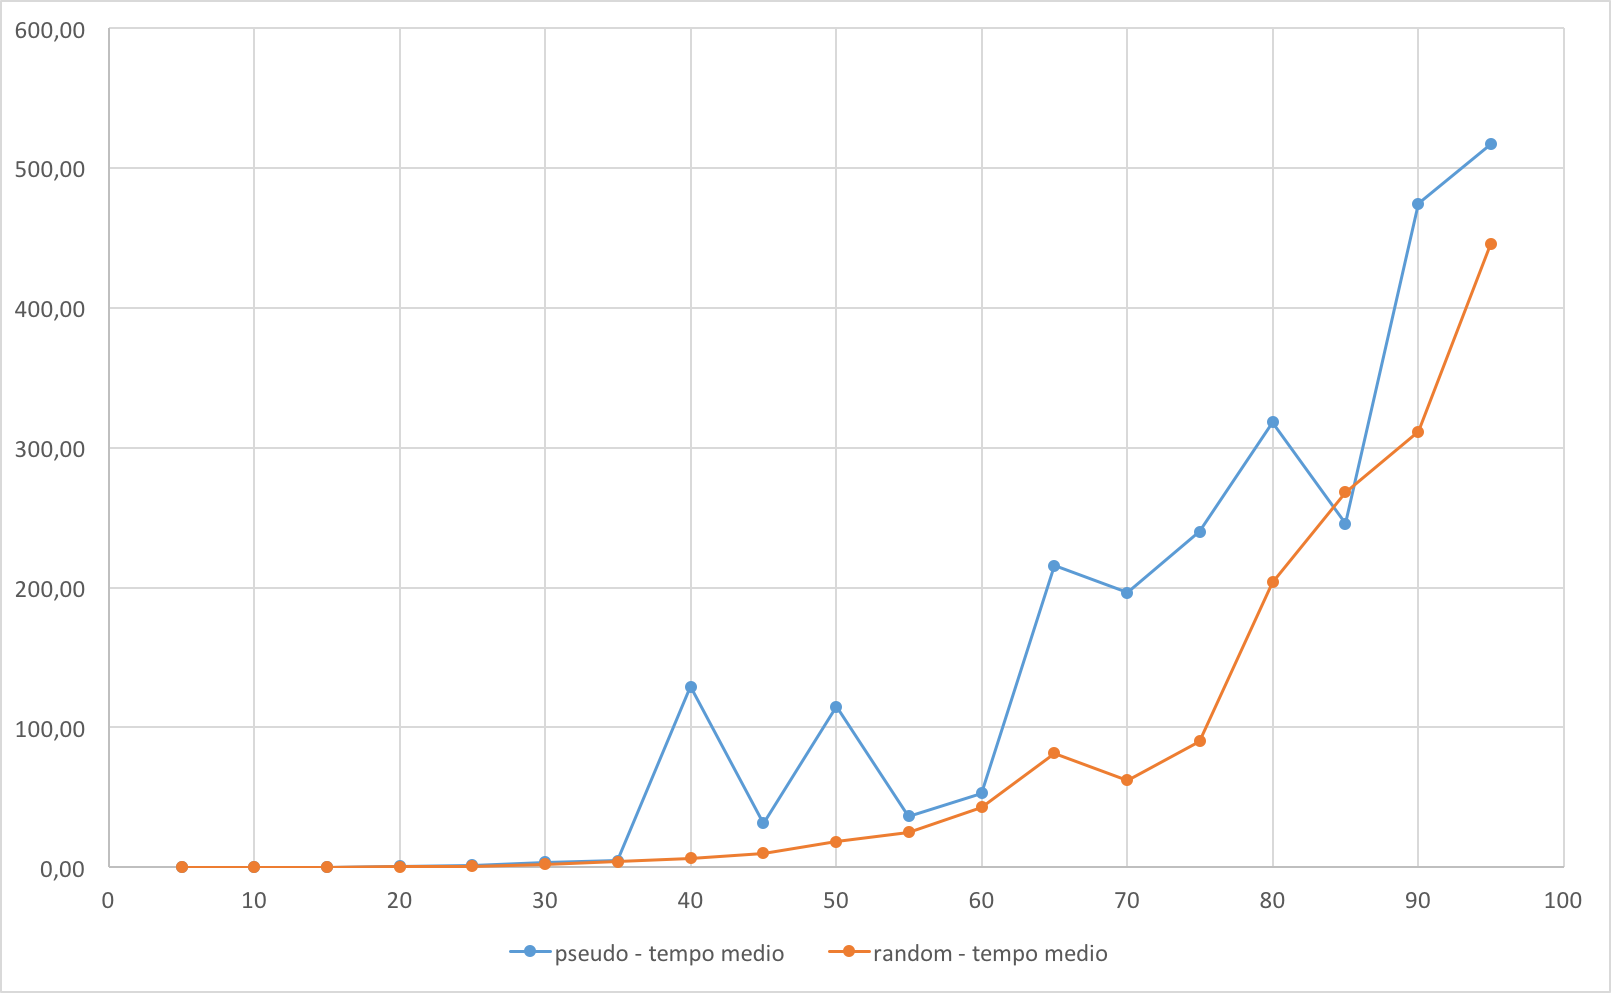
\includegraphics[width=.9\textwidth]{immagini/cplex-time.png}
	\caption{Tempo medio impiegato da CPLEX per risolvere le varie istanze}\label{fig:cplex-time}
\end{figure}

\begin{table}[htbp]
	\centering
	\begin{tabular}{c|c|c|}
		\cline{2-3}
		& \multicolumn{2}{c|}{\textbf{Dimensione}} \\ \hline
		\multicolumn{1}{|c|}{\textbf{Time limit} (s)} & \textbf{Pseudo}      & \textbf{Rand}     \\ \hline
		\multicolumn{1}{|c|}{1}                   & 20                   & 25                \\ \hline
		\multicolumn{1}{|c|}{10}                  & 35                   & 45                \\ \hline
		\multicolumn{1}{|c|}{60}                  & 60                   & 60                \\ \hline
		\multicolumn{1}{|c|}{600}                 & 85                   & 95               \\ \hline
	\end{tabular}
	\caption{Massima difficoltà mediamente risolvibile entro i rispettivi time limit. Per determinare la difficoltà è stata usata la media, senza prendere in considerazione i casi limite in cui già per $N$ bassi non viene trovata una soluzione.}
	\label{tab:cplex-recap}
\end{table}

Dai risultati ottenuti si può osservare che:

\begin{itemize}
	\item Le istanze generate casualmente sembrano essere mediamente più facili da risolvere rispetto a quelle generate in modo pseudo casuale.
	\item Per quanto riguarda le istanze pseudo casuali, già con $N=40$ è stata trovata un'istanza che CPLEX non riesce a risolvere entro 10 minuti d'esecuzione.
	\item Con $N = 100$ solo due istanze di quelle generate casualmente è sono state risolte, mentre di quelle pseudo casuali non ne è stata risolta nessuna. Pertanto sembra che la distribuzione dei punti sia notevolmente influente sulle prestazioni dell'algoritmo.
\end{itemize}
		% Descrizione della struttura del programma
	% !TEX encoding = UTF-8
% !TEX program = pdflatex
% !TEX root = relazione-MEMOC.tex
% !TeX spellcheck = it_IT

\FloatBarrier
\section{Algoritmo Genetico}\label{sec:genetico}

Come meta-euristica ad-hoc si è scelto di implementare un algoritmo genetico seguendo le indicazioni presenti nelle dispense del corso.

\subsection{Scelte progettuali}

Gli algoritmi genetici lasciano molte possibilità di scelta al progettatore e le scelte effettuate influenzano notevolmente l'efficacia e efficienza dell'algoritmo.

Nel determinare i vari componenti si è cercato di progettare un algoritmo bilanciato, che parta da delle soluzioni buone, ma che converga lentamente grazie alle mutazioni e alla selezione di Montecarlo.

\subsubsection{Codifica delle soluzioni}

Per la codifica delle soluzioni si è scelto di utilizzare un'array di lunghezza $N+1$, dove $N$ è il numero di nodi da visitare o fori da effettuare, che rappresenta la sequenza in cui vengono visitati i nodi. La dimensione dell'array è di $N+1$ perché viene aggiunto un ultimo elemento sempre fisso a $0$ per imporre il vincolo che la trivella ritorni al punto di partenza.
Allo stesso modo è imposto il vincolo che il primo elemento dell'array sia 0, in modo che il nodo di partenza sia sempre quello e che coincida con il nodo finale. Un esempio della codifica è disponibile in figura \ref{fig:rappr}.

\begin{figure}[htbp]
	\centering
	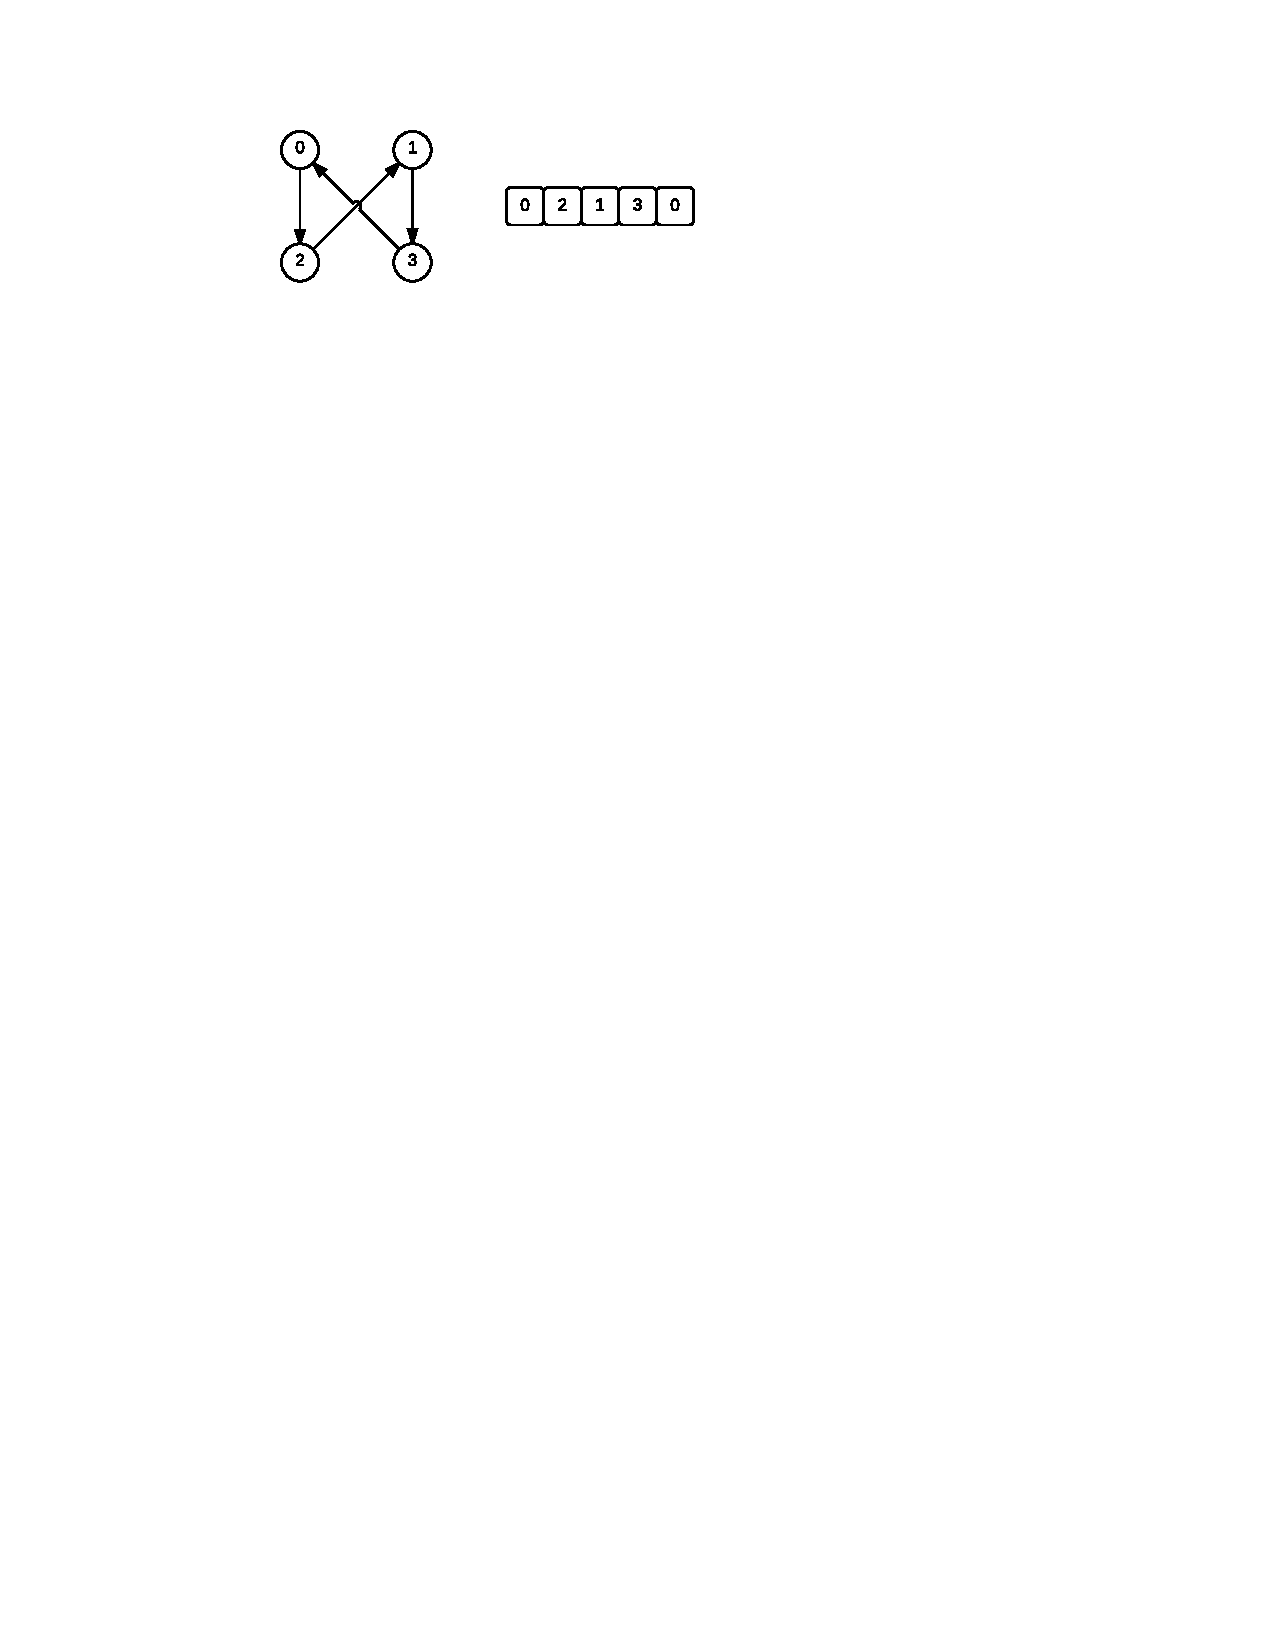
\includegraphics[width=.6\textwidth]{immagini/path-rappr.pdf}
	\caption{Possibile percorso su un grafo di 4 nodi con la relativa rappresentazione interna.}\label{fig:rappr}
\end{figure}

\subsubsection{Generazione della popolazione iniziale}

La popolazione iniziale viene creata con delle soluzioni generate in modo pseudo-greedy.
Ovvero, ogni soluzione viene generata incrementalmente a partire dal nodo di partenza, andando a scegliere come nodo successivo un nodo qualsiasi tra quelli ancora da visitare.
La scelta del nodo viene effettuata casualmente, dando una maggiore probabilità di essere scelti ai nodi migliori.

Per quanto riguarda la dimensione della popolazione, si è scelto di implementarla come parametro dell'algoritmo, in modo che sia possibile specificare una dimensione diversa in base alla dimensione delle istanze che l'algoritmo si troverà a risolvere.
Questo perché è ragionevole assumere che istanze di grandi dimensioni abbiano un numero maggiore di possibili soluzioni e quindi poter specificare una dimensione \textit{ad-hoc} permette di avere una popolazione sufficientemente grande da rappresentare un campione significativo delle possibili soluzioni.

\subsubsection{Funzione di fitness}

Come funzione di fitness per gli individui è stata utilizzata la funzione obiettivo, ovvero il costo del ciclo descritto dalla soluzione.

\subsubsection{Operatore di selezione}

La selezione delle soluzioni da riprodurre viene effettuata secondo un \textit{torneo-K}. Vengono scelti casualmente dalla popolazione $K$ individui, con $K = \texttt{POPULATION\_SIZE}/10$ e tra questi viene scelto il miglior candidato per partecipare alla riproduzione.
Il processo viene quindi eseguito due volte in modo da scegliere i due genitori.

\subsubsection{Crossover}

Il crossover viene effettuato in modo uniforme utilizzando i due genitori precedentemente scelti, dando maggior probabilità di esser trasmessi ai geni del genitore migliore.
La combinazione dei geni viene effettuata costruendo un nuovo cammino a partire dagli archi presenti nei cammini dei due genitori.

Sia $succ(x, G)$ il nodo successivo al nodo $x$ nel cammino della soluzione $G$, pertanto nella soluzione $G$ sarà presente l'arco $(x, succ(x,G))$ e siano $G_1$ e $G_2$ i due genitori della nuova soluzione.

Si ha quindi che la costruzione del nuovo cammino partirà dal nodo 0 e che il secondo nodo del cammino verrà scelto casualmente tra $succ(0,G_1)$ e $succ(0,G_2)$.
Al passo successivo, l'ultimo nodo inserito nel nuovo cammino sarà un nodo $y$ e pertanto la scelta del nodo su cui spostarsi sarà tra $succ(y,G_1)$ o $succ(y, G_2)$.
Il procedimento viene ripetuto finché non sarà completato il ciclo, tornando al nodo 0.

Durante la costruzione del figlio possono capitare alcuni casi particolari:

\begin{itemize}
	\item Uno dei due possibili successori è già presente nel cammino. In questo caso viene scelto l'altro.
	\item Entrambi i nodi fanno già parte del cammino. Il questo caso come successore viene scelto il nodo migliore tra quelli disponibili.
	\item Il nodo finale del cammino deve essere il nodo 0. Quindi l'ultimo arco viene scelto forzatamente in modo che sia verso il nodo 0.
\end{itemize}

Da notare che per come sono gestiti questi casi particolari non possono essere generate soluzioni non ammissibili.

\subsubsection{Mutazione}

\`E stata prevista la possibilità che durante l'evoluzione delle popolazione alcune soluzioni subiscano una mutazione.

Una mutazione consiste nel rimescolare l'ordine di visita dei nodi interni del ciclo. In questo modo la mutazione viene fatta velocemente e non invalida la soluzione, perché il primo e l'ultimo nodo vistato sarà sempre il nodo 0.

\subsubsection{Sostituzione della popolazione}

La sostituzione delle popolazione viene effettuata generando prima un numero $R$ di individui proporzionale alla dimensione della popolazione. Dopodiché la popolazione viene riportata alla dimensione di partenza, selezionando con il metodo di Montecarlo $N$ soluzioni tra le $N+R$ disponibili.

\subsubsection{Criterio di arresto}

Come criterio d'arresto è stato utilizzato un tempo limite d'esecuzione che può essere specificato all'avvio dell'algoritmo.

La scelta è ricaduta su questa condizione d'arresto perché così risulta più semplice effettuare il confronto con CPLEX e perché l'altro criterio provato, ovvero fermare l'algoritmo dopo $k$ iterazioni che non hanno migliorato la miglior soluzione, richiedeva troppo tempo d'esecuzione a causa del metodo di sostituzione della popolazione.
Infatti, tra un'iterazione e l'altra può essere scartata anche la soluzione migliore e quindi l'iterazione successiva poteva risultare migliorativa anche se in realtà non lo era.

Un altro criterio d'arresto preso in considerazione è stato un limite sulle iterazioni, ma facendo le varie prove si è osservato che è preferibile impostare un tempo limite fisso piuttosto che il numero massimo di iterazioni.

\subsection{Parametri dell'algoritmo e processo di ottimizzazione}

L'algoritmo così implementato richiede che siano specificati i seguenti parametri:

\begin{itemize}
	\item\texttt{POPULATION\_SIZE}: dimensione della popolazione;
	\item\texttt{MUTATION\_RATE}: probabilità di mutazione:
	\item\texttt{GROWTH\_RATIO}: soluzioni generate ad ogni iterazione;
	\item\texttt{TIME\_LIMIT}: tempo limite per l'esecuzione dell'algoritmo.
\end{itemize}

\subsubsection{Esperimenti per l'ottimizzazione dei parametri}

Prima di testare l'algoritmo genetico in modo analogo a quanto fatto per il modello CPLEX è stata eseguita una leggera ottimizzazione dei parametri.

Si sono quindi provate le varie possibili combinazioni dei parametri nella risoluzione di varie istanze di dimensioni diverse (50, 100, 150 punti) generate sia in modo casuale che pseudo-casuale.
Le varie prove sono state poi ripetute 5 volte ed è stata effettuata una media dei risultati.

I valori per i parametri che sono stati provati sono:

\begin{itemize}
	\item \texttt{POPULATION\_SIZE}: 100, 250, 500;
	\item \texttt{MUTATION\_RATE}: 0.01, 0.05, 0.1;
	\item \texttt{GROWTH\_RATIO}: 1.1, 1.5, 2;
	\item \texttt{TIME\_LIMIT}: 1 minuto.
\end{itemize}

Si è scelto di mantenere un \texttt{TIME\_LIMIT} costante e limitato per rendere più agevole la pianificazione delle esecuzioni e allo stesso tempo per limitare la durata degli esperimenti. Infatti, fissato un $N$, per provare tutte e 9 le possibili combinazioni dei parametri, ripetendo la prova 5 volte per ogni istanza, sono necessarie $1350$ esecuzioni, ovvero circa un giorno d'esecuzione.

Di ogni esecuzione è stata tenuta traccia:
\begin{itemize}
	\item della soluzione peggiore;
	\item della soluzione migliore;
	\item dello stato della popolazione, ovvero il fitness medio;
	\item del numero di iterazioni effettuate.
\end{itemize}

mentre per scegliere la configurazione migliore è stata tenuta in considerazione la media di questi valori per le 5 esecuzioni sulla stessa istanza.

\subsubsection{Risultati}

Dall'esecuzione delle prove è emerso che per tutte e tre le possibili dimensioni i risultati migliori si ottengono con \texttt{GROWTH\_RATIO} $= 2$, ovvero andando a generare ad ogni iterazione un numero di individui pari al doppio di quello della popolazione. 
Per quanto riguarda gli altri parametri si è visto che per $N = 100$ e $N = 150$, la configurazione migliore è \texttt{POPULATION\_SIZE} $ = 500$  e \texttt{MUTATION\_RATE} $ = 0.1$ mentre per $N=50$ è \texttt{POPULATION\_SIZE} $ = 100$ e \texttt{MUTATION\_RATE} $ = 0.05$. 

Questa discrepanza può essere dovuta al fatto che all'aumentare della dimensione del grafo si ha un'esplosione combinatoria delle possibili soluzioni e quindi la dimensione della popolazione deve aumentare di conseguenza.

Per quanto riguarda il valore di \texttt{MUTATION\_RATE}, una possibile motivazione per la differenza deriva dal fatto che con $N=50$ l'algoritmo riesce a fare più iterazioni, mentre con un $N$ maggiori ne vengono fatte meno di 10 per ogni istanza e quindi l'effetto delle mutazioni, combinato alla dimensione della popolazione più grande (500 per $N=100$ e $N=150$), risulta più efficace nel produrre soluzioni migliori rispetto all'avanzamento generazionale. 
Questo perché, considerando una popolazione di 500 individui con probabilità di mutazione del $10\%$, in un'iterazione l'effetto dell'avanzamento produce una nuova generazione con un fitness leggermente migliore, mentre la mutazione di $50$ individui, essendo completamente casuale, può generare fin da subito un super-individuo con un elevato fitness.

Un'ultima osservazione riguarda alcune esecuzioni dell'algoritmo con istanze di dimensione $N=150$, le quali hanno avuto un comportamento inatteso. 
Ovvero, mentre la maggior parte delle esecuzioni riusciva a fare solamente un'iterazione a causa del tempo limite di un minuto, le ultime esecuzione hanno fatto in media 15 iterazioni. Tale anomalia può essere legata a come il sistema operativo ha assegnato la CPU al programma, anche se tutte le esecuzioni sono state effettuate sullo stesso computer e in condizioni simili. Per motivi di tempo non è stato poi possibile rieseguire l'algoritmo su tali istanze.

Infine, dato la dimensione consistente delle tabelle, queste non sono riportate nella relazione, ma sono contenute in un file Excel presente all'interno dell'archivio consegnato assieme alla relazione.

\subsection{Test dell'algoritmo}

Per testare l'algoritmo genetico sono state utilizzate le stesse istanze utilizzate per il modello CPLEX, in modo da poter calcolare anche l'optimality gap ottenuto dall'algoritmo genetico.

Come parametri dell'algoritmo sono stati utilizzati:

\begin{itemize}
	\item \texttt{POPULATION\_SIZE}: 100;
	\item \texttt{MUTATION\_RATE}: 0.05;
	\item \texttt{GROWTH\_RATIO}: 2.
\end{itemize}

\noindent Ovvero quelli che sono risultati migliori dal processo di ottimizzazione.

L'algoritmo è stato eseguito 5 volte per ogni istanza e poi è stata presa in considerazione la media dei risultati. 
Inoltre, per ridurre il tempo necessario è stato assegnato come limite temporale per la durata dell'esecuzione dell'algoritmo genetico la stessa soglia temporale che ha utilizzato CPLEX\footnote{Fatta eccezione per la soglia da 10 minuti, in quanto si è visto che già con 5 minuti l'algoritmo convergeva ad una soluzione.}.
I vari limiti temporali per le istanze sono quindi simili a quelli riportati in tabella \ref{tab:cplex-recap}.

I risultati ottenuti sono riportati in tabella \ref{tab:ga-recap}, mentre il grafico in figura \ref{fig:ga-gap} rappresenta il deterioramento dell'optimality gap al crescere della dimensione del problema.

\begin{table}[htbp]
	\centering
	\resizebox{\textwidth}{!}{%
		\begin{tabular}{c|c|c|c|c|c|c|}
			\cline{2-7}
			\multicolumn{1}{l|}{} & \multicolumn{3}{c|}{\textbf{Pseudo}} & \multicolumn{3}{c|}{\textbf{Random}} \\ \hline
			\multicolumn{1}{|c|}{\textbf{Dimensione}} & \textbf{\begin{tabular}[c]{@{}c@{}}Tempo\\ Medio (s)\end{tabular}} & \textbf{\begin{tabular}[c]{@{}c@{}}Valore\\ Medio\end{tabular}} & \textbf{\begin{tabular}[c]{@{}c@{}}Media\\ Gap ottimo (\%)\end{tabular}} & \textbf{\begin{tabular}[c]{@{}c@{}}Tempo\\ Medio (s)\end{tabular}} & \textbf{\begin{tabular}[c]{@{}c@{}}Valore\\ Medio\end{tabular}} & \textbf{\begin{tabular}[c]{@{}c@{}}Media\\ Gap ottimo (\%)\end{tabular}} \\ \hline
			\multicolumn{1}{|c|}{5} & 0,99 & 13,55 & 0,00 & 0,97 & 17,27 & 0,00 \\ \hline
			\multicolumn{1}{|c|}{10} & 1,00 & 35,59 & 5,88 & 1,00 & 53,04 & 11,16 \\ \hline
			\multicolumn{1}{|c|}{15} & 1,00 & 48,23 & 11,50 & 1,00 & 73,63 & 17,59 \\ \hline
			\multicolumn{1}{|c|}{20} & 1,00 & 77,97 & 27,56 & 1,00 & 119,13 & 24,07 \\ \hline
			\multicolumn{1}{|c|}{25} & 10,00 & 121,55 & 31,57 & 10,00 & 170,29 & 30,38 \\ \hline
			\multicolumn{1}{|c|}{30} & 10,00 & 100,59 & 40,66 & 10,00 & 202,44 & 34,97 \\ \hline
			\multicolumn{1}{|c|}{35} & 10,00 & 125,34 & 41,44 & 10,00 & 274,39 & 31,11 \\ \hline
			\multicolumn{1}{|c|}{40} & 59,97 & 217,40 & 33,24$^*$ & 60,00 & 263,47 & 36,49 \\ \hline
			\multicolumn{1}{|c|}{45} & 60,00 & 182,59 & 29,96 & 60,00 & 347,77 & 41,80 \\ \hline
			\multicolumn{1}{|c|}{50} & 60,00 & 295,67 & 36,56 & 59,99 & 508,70 & 35,76 \\ \hline
			\multicolumn{1}{|c|}{55} & 60,00 & 469,33 & 44,11 & 59,99 & 509,22 & 44,20 \\ \hline
			\multicolumn{1}{|c|}{60} & 60,00 & 384,25 & 45,73 & 59,99 & 574,03 & 38,59 \\ \hline
			\multicolumn{1}{|c|}{65} & 60,00 & 433,19 & 44,12$^*$ & 59,99 & 766,07 & 37,90 \\ \hline
			\multicolumn{1}{|c|}{70} & 300,00 & 504,16 & 55,30$^*$ & 299,94 & 821,45 & 43,62 \\ \hline
			\multicolumn{1}{|c|}{75} & 300,00 & 470,13 & 55,53 & 299,99 & 1010,75 & 42,60 \\ \hline
			\multicolumn{1}{|c|}{80} & 299,99 & 475,65 & 50,26$^*$ & 300,00 & 777,70 & 39,96 \\ \hline
			\multicolumn{1}{|c|}{85} & 299,99 & 911,71 & 52,62$^*$ & 299,97 & 898,70 & 44,70 \\ \hline
			\multicolumn{1}{|c|}{90} & 299,99 & 684,37 & 44,29$^*$ & 299,99 & 1211,12 & 45,72$^*$ \\ \hline
			\multicolumn{1}{|c|}{95} & 299,99 & 1029,86 & 60,11$^*$ & 299,99 & 1032,96 & 50,15$^*$ \\ \hline
			\multicolumn{1}{|c|}{100} & 299,99 & 834,27 & - & 299,99 & 1071,50 & - \\ \hline
		\end{tabular}%
	}
	\caption{Risultati ottenuti dall'esecuzione dell'algoritmo genetico sulle istanze di benchmark. Per ogni dimensione sono state provate 5 istanze diverse e l'algoritmo è stato eseguito su ogni istanza 5 volte. Per $N=100$ non è presente l'optimality gap in quanto CPLEX non è riuscito a risolvere entro il tempo limite le istanze. Alcuni valori del gap dall'ottimo sono marcati con $^*$ perché per alcune delle istanze così marcate, CPLEX non è riuscito a completare l'esecuzione in tempo e quindi ha fornito una soluzione ammissibile ma che non è garantito essere ottima.}
	\label{tab:ga-recap}
\end{table}

\begin{figure}[htbp]
	\centering
	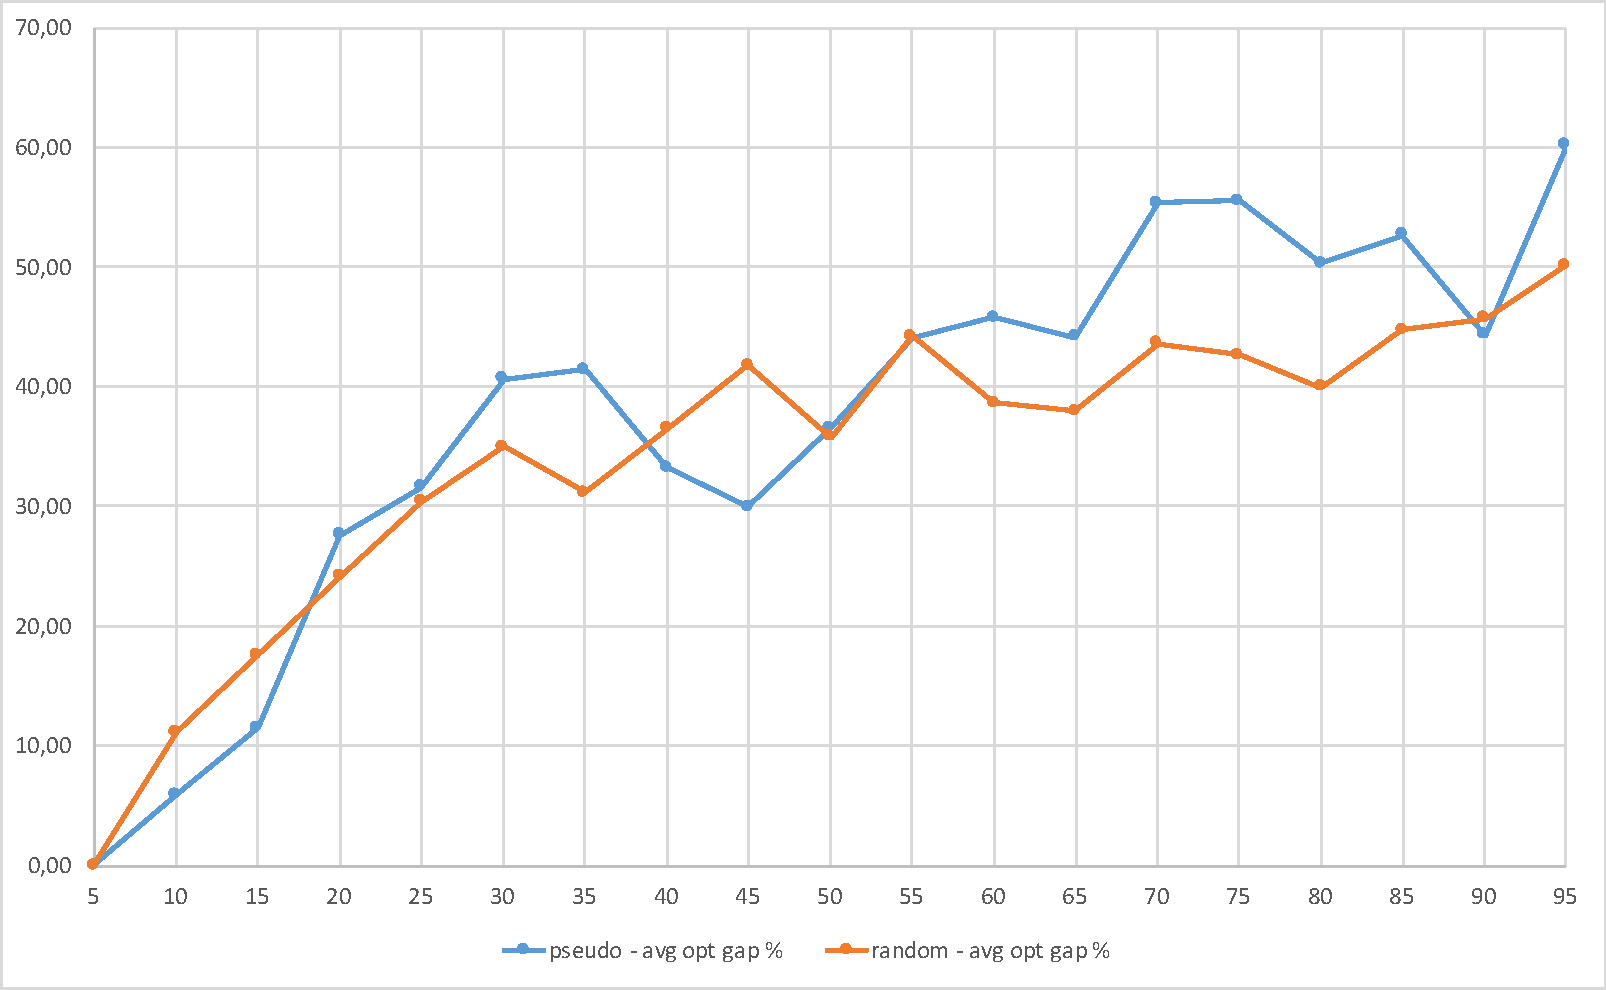
\includegraphics[width=\textwidth]{immagini/ga-opt-gap.pdf}
	\caption{Gap tra la soluzione ottima del problema e la migliore soluzione trovata dall'algoritmo genetico al crescere di $N$}\label{fig:ga-gap}
\end{figure}

Dai risultati riportati si può osservare che:

\begin{itemize}
	\item Le prestazioni dell'algoritmo genetico, in quanto ad optimality gap, sono simili sia che vengano risolte istanze generate casualmente, che istanze pseudo-casuali. \item Dalla figura \ref{fig:ga-gap} si può notare che al crescere di $N$, l'optimality gap risulta essere leggermente migliore per le istanze casuali, questo sembra confermare quando osservato con CPLEX, ovvero che le istanze generate casualmente siano più semplici da risolvere.
	\item Le prestazioni dell'algoritmo sono comunque scadenti e questo può essere legato ad una convergenza troppo veloce della popolazione verso un'unica tipologia di soluzioni. Un'analisi più approfondita di ciò è presente nella seguente sezione.
	\item Anche per istanze di piccole dimensioni vengono prodotte delle soluzioni particolarmente scadenti. Questo può essere dovuto al fatto che il tempo limite imposto sia troppo stretto e che non permetta all'algoritmo genetico di effettuare un numero sufficiente di iterazioni.
\end{itemize}

\subsubsection{Analisi della convergenza e delle prestazioni}

Andando a monitorare l'esecuzione dell'algoritmo genetico, si è osservato che tipicamente la convergenza ad una determinata soluzione viene raggiunta con 1000 iterazioni, mentre con i parametri attuali e con un limite d'esecuzione di 5 minuti, l'algoritmo riesce a fare circa 3000 iterazioni\footnote{Per questo motivo il limite temporale è stato ridotto da 10 minuti a 5.}.

Pertanto ci sono ampi margini di miglioramento per le prestazioni dell'algoritmo genetico, andando ad ottimizzare in modo migliore i parametri e a modificare alcune scelte progettuali.
Questo risultato era aspettato in quanto le criticità degli algoritmi genetici sono le svariate scelte progettuali che si possono effettuare e l'elevato numero di parametri da ottimizzare.

Per questo progetto le scelte progettuali sono state legate per lo più alla semplicità, in modo che fosse più semplice individuare e risolvere eventuali errori implementativi e, allo stesso tempo, l'ottimizzazione dei parametri è stata ridotta a causa dei vincoli temporali. 
Quest'ultimo vincolo può aver influenzato l'ottimizzazione perché, con un limite di un minuto ad esecuzione, i valori per i parametri che rendono veloce l'esecuzione dell'algoritmo, e quindi permettono di fare più iterazioni nello stesso tempo, possono risultare migliori rispetto ad altri valori che ne rallentano l'esecuzione, diminuendo di conseguenza il numero di iterazioni, mentre con un tempo d'esecuzione maggiore, questi secondi valori potrebbero essere risultati migliori.

Visti i risultati ottenuti, si possono individuare alcune modifiche dell'algoritmo che potrebbero portare a dei risultati migliori:

\begin{itemize}
	\item \textbf{Generazione e dimensione della popolazione}: anziché utilizzare una dimensione costante, la si può rendere proporzionale alla dimensione del problema. In questo modo si ha un pool di soluzioni iniziali che è sempre sufficientemente grande.
	Sempre per diversificare ulteriormente la popolazione è possibile generare le soluzioni in modo casuale, anziché costruirle con un euristica pseudo-greedy.
	\item \textbf{Operazione di crossover}: la combinazione di due soluzioni utilizza un'approccio greedy per completare la soluzione figlia, andando a forzare la struttura della nuova generazione. Un approccio alternativo che potrebbe diversificare maggiormente la nuova generazione è quello di andare ad aggiungere i nodi mancanti per completare il percorso in ordine casuale. Così facendo si ha comunque la certezza che la nuova soluzione sia ammissibile.
	\item \textbf{Distanza di Hamming}: sia per valutare il fitness di una soluzione, che per sostituire la popolazione, può essere presa in considerazione la distanza di Hamming tra tutte le coppie di soluzioni presenti nella popolazione. Così facendo si può aumentare il fitness di una soluzione che è mediamente più diversa dalle altre e allo stesso tempo si può cercare di mantenere una certa diversificazione quando vengono scelte le soluzioni da mantenere nella popolazione.
\end{itemize}

Da notare che l'implementazione del primo e terzo punto vanno ad aumentare il carico computazionale dell'algoritmo e quindi il numero di iterazioni sarà quasi sicuramente inferiore a 3000.

Per bilanciare questo aumento di carico computazionale si potrebbero andare a dividere l'esecuzione di alcune operazioni su più thread. 
Infatti, CPLEX ha il vantaggio implementativo di sfruttare contemporaneamente più core della CPU, mentre l'algoritmo genetico implementato è sequenziale, quando in realtà la generazione delle soluzioni iniziali, così come l'evoluzione della popolazione e l'eventuale calcolo della distanza di Hamming tra le coppie di soluzioni, potrebbero essere distribuite su più thread.

















		% Problemi implementativi
	% !TEX encoding = UTF-8
% !TEX program = pdflatex
% !TEX root = relazione-MEMOC.tex
% !TeX spellcheck = it_IT

\section{Confronto} \label{sec:confronto}

    % Descrizione degli esperimenti
	% !TEX encoding = UTF-8
% !TEX program = pdflatex
% !TEX root = relazione-MEMOC.tex
% !TeX spellcheck = it_IT

\section{Conclusioni}

Il modello CPLEX è risultato nettamente superiore all'algoritmo genetico, principalmente perché le istanze sulle quali è stato eseguito erano di dimensione ridotte. 
Nel caso pratico ci sono schede con molti più fori e quindi trovare una soluzione ottima potrebbe richiedere molto più di 10 minuti.

D'altro canto l'algoritmo genetico ora come ora, non è una grande alternativa in quanto il gap dalla soluzione ottima è considerevole. 
In ogni caso, la certezza dell'ottimalità con l'algoritmo genetico non si può avere, ma le modifiche suggerite potrebbero fornire soluzioni migliori rispetto a quelle attuali.

C'è poi un'altra considerazione da fare riguardo la distribuzione dei fori nella scheda, che nel caso pratico sono tra loro raggruppati in insiemi di fori vicini.
Si è cercato di imitare ciò con le istanze pseudo-casuali e si è osservato che al crescere del numero dei fori, sia il modello CPLEX che l'algoritmo genetico, fanno più fatica a risolvere tali istanze.
Questo può essere dovuto al fatto che il modello CPLEX ``\textit{perda tempo}'' ad ottimizzare lo spostamento all'interno dei vari gruppi, mentre per l'algoritmo genetico vengono creati più minimi locali ai quali converge la popolazione.
Pertanto un algoritmo euristico alternativo potrebbe prima risolvere il problema principale, ovvero trovare il ciclo ottimo che permette di visitare tutti i vari gruppi di fori da effettuare e poi ottimizzare il percorso interno di ciascuno gruppo.
Così facendo si scompone il problema in più sotto-problemi con meno variabili e quindi più veloci da risolvere. 
Inoltre, è ragionevole pensare che la parte più critica sia l'ordine in cui vengono visitati i vari gruppi di fori, perché questi possono essere più sparsi, mentre l'ordine in cui vengono effettuati i fori che appartengono ad uno stesso insieme risulta meno importante perché sono tra loro vicini.
Si può quindi progettare un approccio ibrido, che usa un modello esatto per calcolare il ciclo ottimo di visita dei vari gruppi e un'euristica per determinare il percorso di foratura interno ai vari insiemi. 



    % Conclusioni
	\appendix						
	% !TEX encoding = UTF-8
% !TEX program = pdflatex
% !TEX root = relazione-MEMOC.tex
% !TeX spellcheck = it_IT

\section{Informazioni sul codice e sulla consegna}

Il codice consegnato è suddiviso in varie sotto-directory:

\begin{itemize}
	\item \texttt{common}: contiene le classi comuni, utilizzate sia dal modello CPLEX che dall'algoritmo genetico.
	\item \texttt{cplex}: contiene le classi relative all'implementazione del modello CPLEX.
	\item \texttt{ga}: contiene le classi relative all'implementazione dell'algoritmo genetico.
\end{itemize}

Il codice è stato poi strutturato in modo simile ad una libreria: per entrambe le parti del progetto c'è una classe che incapsula l'algoritmo risolutivo e che espone un metodo \texttt{solve()}.
Pertanto non è presente un vero e proprio file principale dell'applicazione.

Vengono però forniti vari file \texttt{.cpp} che contengo degli esempi di utilizzo della libreria e che corrispondo ai programmi utilizzati per eseguire i test.
Viene anche fornito un \texttt{main.cpp} che risolve in entrambi i modi un'istanza di un problema generata casualmente. Tale programma può essere compilato utilizzando il comando \texttt{make}.
All'interno del \texttt{Makefile} sono definite anche le regole per compilare gli altri sorgenti.


\subsection{Possibili problemi di compilazione}

Il programma \texttt{main.cpp}, e di conseguenza tutto il codice prodotto, compilano correttamente sui computer del laboratorio con \texttt{g++ v5.4}.
Tuttavia potrebbero esserci dei problemi nel linking delle librerie di CPLEX. In questo caso è necessario andare ad aggiustare il \textit{filepath} definiti all'interno del \texttt{Makefile}.
		% Come eseguire il codice
	%----------------------------------------------------------------------------------------
	%	CONTENT
	%----------------------------------------------------------------------------------------
	
	
\end{document}